\documentclass[12pt,a4paper]{article}

% --- Pakiety ---
\usepackage[utf8]{inputenc}
\usepackage[T1]{fontenc}
\usepackage[polish]{babel}
\usepackage{geometry}
\usepackage{xcolor}
\usepackage{enumitem}
\usepackage{titlesec}
\usepackage{helvet}

\usepackage[hidelinks]{hyperref}

\renewcommand{\familydefault}{\sfdefault}
\usepackage{tikz}

% --- Konfiguracja strony ---
\geometry{left=0.cm, top=1cm, right=0.3cm, bottom=0.1cm}
\pagestyle{empty}

% --- Poprawione kolory ---
\definecolor{headerblue}{RGB}{9, 56, 102}   
\definecolor{sidebarlightblue}{RGB}{230, 236, 242} 
\definecolor{textdark}{RGB}{40, 40, 40}
\definecolor{sectioncolor}{RGB}{9, 56, 102}

% --- Styl sekcji ---
% Zastosowanie koloru do sekcji
\titleformat{\section}
{\large\bfseries\color{sectioncolor}} %kolor tekstu
{}
{0pt}
{}
[{\color{sectioncolor}\titlerule[1pt]}] %kolor linii pod tekstem
\titlespacing*{\section}{0pt}{10pt}{5pt}

\begin{document}

% --- TŁO ---
\begin{tikzpicture}[remember picture, overlay]
    % Szary prostokąt z prawej (35%  szerokości strony)
    \fill[sidebarlightblue] ([xshift=-8.5cm]current page.north east) rectangle (current page.south east);
    % Niebieski prostokąt na górze
    \fill[headerblue] (current page.north west) rectangle ([yshift=-1.8cm]current page.north east);
   
\end{tikzpicture}

% --- TREŚĆ NAGŁÓWKA ---
\begin{minipage}[t][-0.5cm][c]{\textwidth}
    \vspace{-0.5cm}
    {\noindent \color{white} \Huge \textbf{Małgorzata Świderek}}
    \vspace{0.8cm}
\end{minipage}

% --- UKŁAD KOLUMN ---
\begin{minipage}[t]{0.54\textwidth} % LEWA KOLUMNA
    \color{textdark}
    \small
    Jestem chętną do nauki studentką III roku na wydziale Informatyki (specjalizacja Data Science) na Polsko-Japońskiej Akademii Technik Komputerowych. Szukam stażu, który pozwoli mi rozwinąć zdobytą na studiach wiedzę w kierunku tworzenia aplikacji opartych o nowoczesne rozwiązania i technologie. Aktualnie jestem w trakcie pisania pracy inżynierskiej na temat "Zastosowanie metod uczenia maszynowego w predykcji oczekiwanej długości życia na podstawie wybranych czynników".
    
    \section*{Doświadczenie projektowe}
    \textbf{GitHub:} \href{https://github.com/s31302}{\color{headerblue}{github.com/s31302}}
    
    \begin{itemize}[leftmargin=*, noitemsep, topsep=2pt]

        \item\textbf{Rozpoznawanie Liter} \textit{Python, Scikit-learn, Pandas, NumPy, Matplotlib, Seaborn, projekt tworzony w zespole dwuosobowym} 
        \href{https://github.com/s31302/rozpoznawanie_liter}{\footnotesize\color{headerblue}{[Kod źródłowy]}}

        \item\textbf{Aplikacja webowa CRUD} \textit{Java, Spring, HTML} 
        \href{https://github.com/s31302/spring-boot-anime-crud}{\footnotesize\color{headerblue}{[Kod źródłowy]}}

        \item\textbf{Mini projekty -  wizja maszynowa} \textit{Python, cv2, numpy, tensorflow, matplotlib} 
        \href{https://github.com/s31302/wma}{\footnotesize\color{headerblue}{[Kod źródłowy]}}

        \item\textbf{Desktopowy system zarządzania z bazą danych} \textit{Java, ORM (np. Hibernate), UML}
        {\footnotesize\color{textdark}{[Projekt akademicki -- kod prywatny ze względu na restrykcje antyplagiatowe]}}
        
        \item\textbf{Gra PacMan} \textit{Java, GUI(Swing)}
        \href{https://github.com/s31302/pac-man}{\footnotesize\color{headerblue}{[Kod źródłowy]}}

        \item\textbf{Gra inspirowana Undertale} \textit{Python, Pygame, Tkinter, projekt tworzony w zespole dwuosobowym}
        \href{https://github.com/s31302/ppy-nightmare}{\footnotesize\color{headerblue}{[Kod źródłowy]}}
        
        \item\textbf{Logo stworzone za pomocą grafiki wektorowej}\textit{Inkscape}
        \href{https://github.com/s31302/kitty-cup-logo}{\footnotesize\color{headerblue}{[Kod źródłowy]}}

        \item\textbf{Interaktywne CV} \textit{LaTeX}
        \href{https://github.com/s31302/cv}{\footnotesize\color{headerblue}{[Kod źródłowy]}}

    \end{itemize}
    
    \section*{Doświadczenie zawodowe}

    \begin{minipage}[c]{0.12\textwidth}
        
\includegraphics[width=\textwidth]{T-Mobile_logo.png}
    \end{minipage}
    \hfill
    \begin{minipage}[c]{0.85\textwidth}
        \textbf{T-Mobile Polska S.A.}\\
        \textit{Pracownik działu administracji HR -- umowa zlecenie}
        07.2024 -- 12.2025 
    \end{minipage}

    \vspace{0.3cm}

    
    \textbf{Zakres obowiązków:}
    \begin{itemize}[leftmargin=*, noitemsep, topsep=2pt]
        \item\textit{Digitalizacja dokumentacji}
        \item\textit{Zarządzanie archiwizacją dokumentacji}
        \item\textit{Przygotowanie dokumentacji gotowej do implementacji do systemu SAP}
        \item\textit{Analiza procesów w kierunku ich optymalizacji}
    \end{itemize}

    \section*{Edukacja}

    \begin{minipage}[c]{0.12\textwidth}
        
\includegraphics[width=\textwidth]{PJATK_logo.png}
    \end{minipage}
    \hfill
    \begin{minipage}[c]{0.85\textwidth}
        \textbf{Polsko-Japońska Akademia Technik Komputerowych (PJATK)}\\
        10.2023 -- obecnie 
    \end{minipage}
    
    \vspace{0.3cm}

    \begin{minipage}[c]{0.12\textwidth}
        
\includegraphics[width=\textwidth]{kollataj_logo.png}
    \end{minipage}
    \hfill
    \begin{minipage}[c]{0.85\textwidth}
        \textbf{XXI Liceum Ogólnokształcące im. Hugona Kołłątaja w Warszawie}\\
        09.2019 -- 04.2023
    \end{minipage}
    
    \section*{Kursy i Certyfikaty}
    \textbf{Umiejętności Jutra AI 3.0 -- Program Szkoleniowy Google} \\
    05.2026 -- obecnie    
    
\end{minipage}
\hfill
\begin{minipage}[t]{0.37\textwidth} % PRAWA KOLUMNA
    \vspace{0cm} 
    \color{textdark}
    
    \centering
    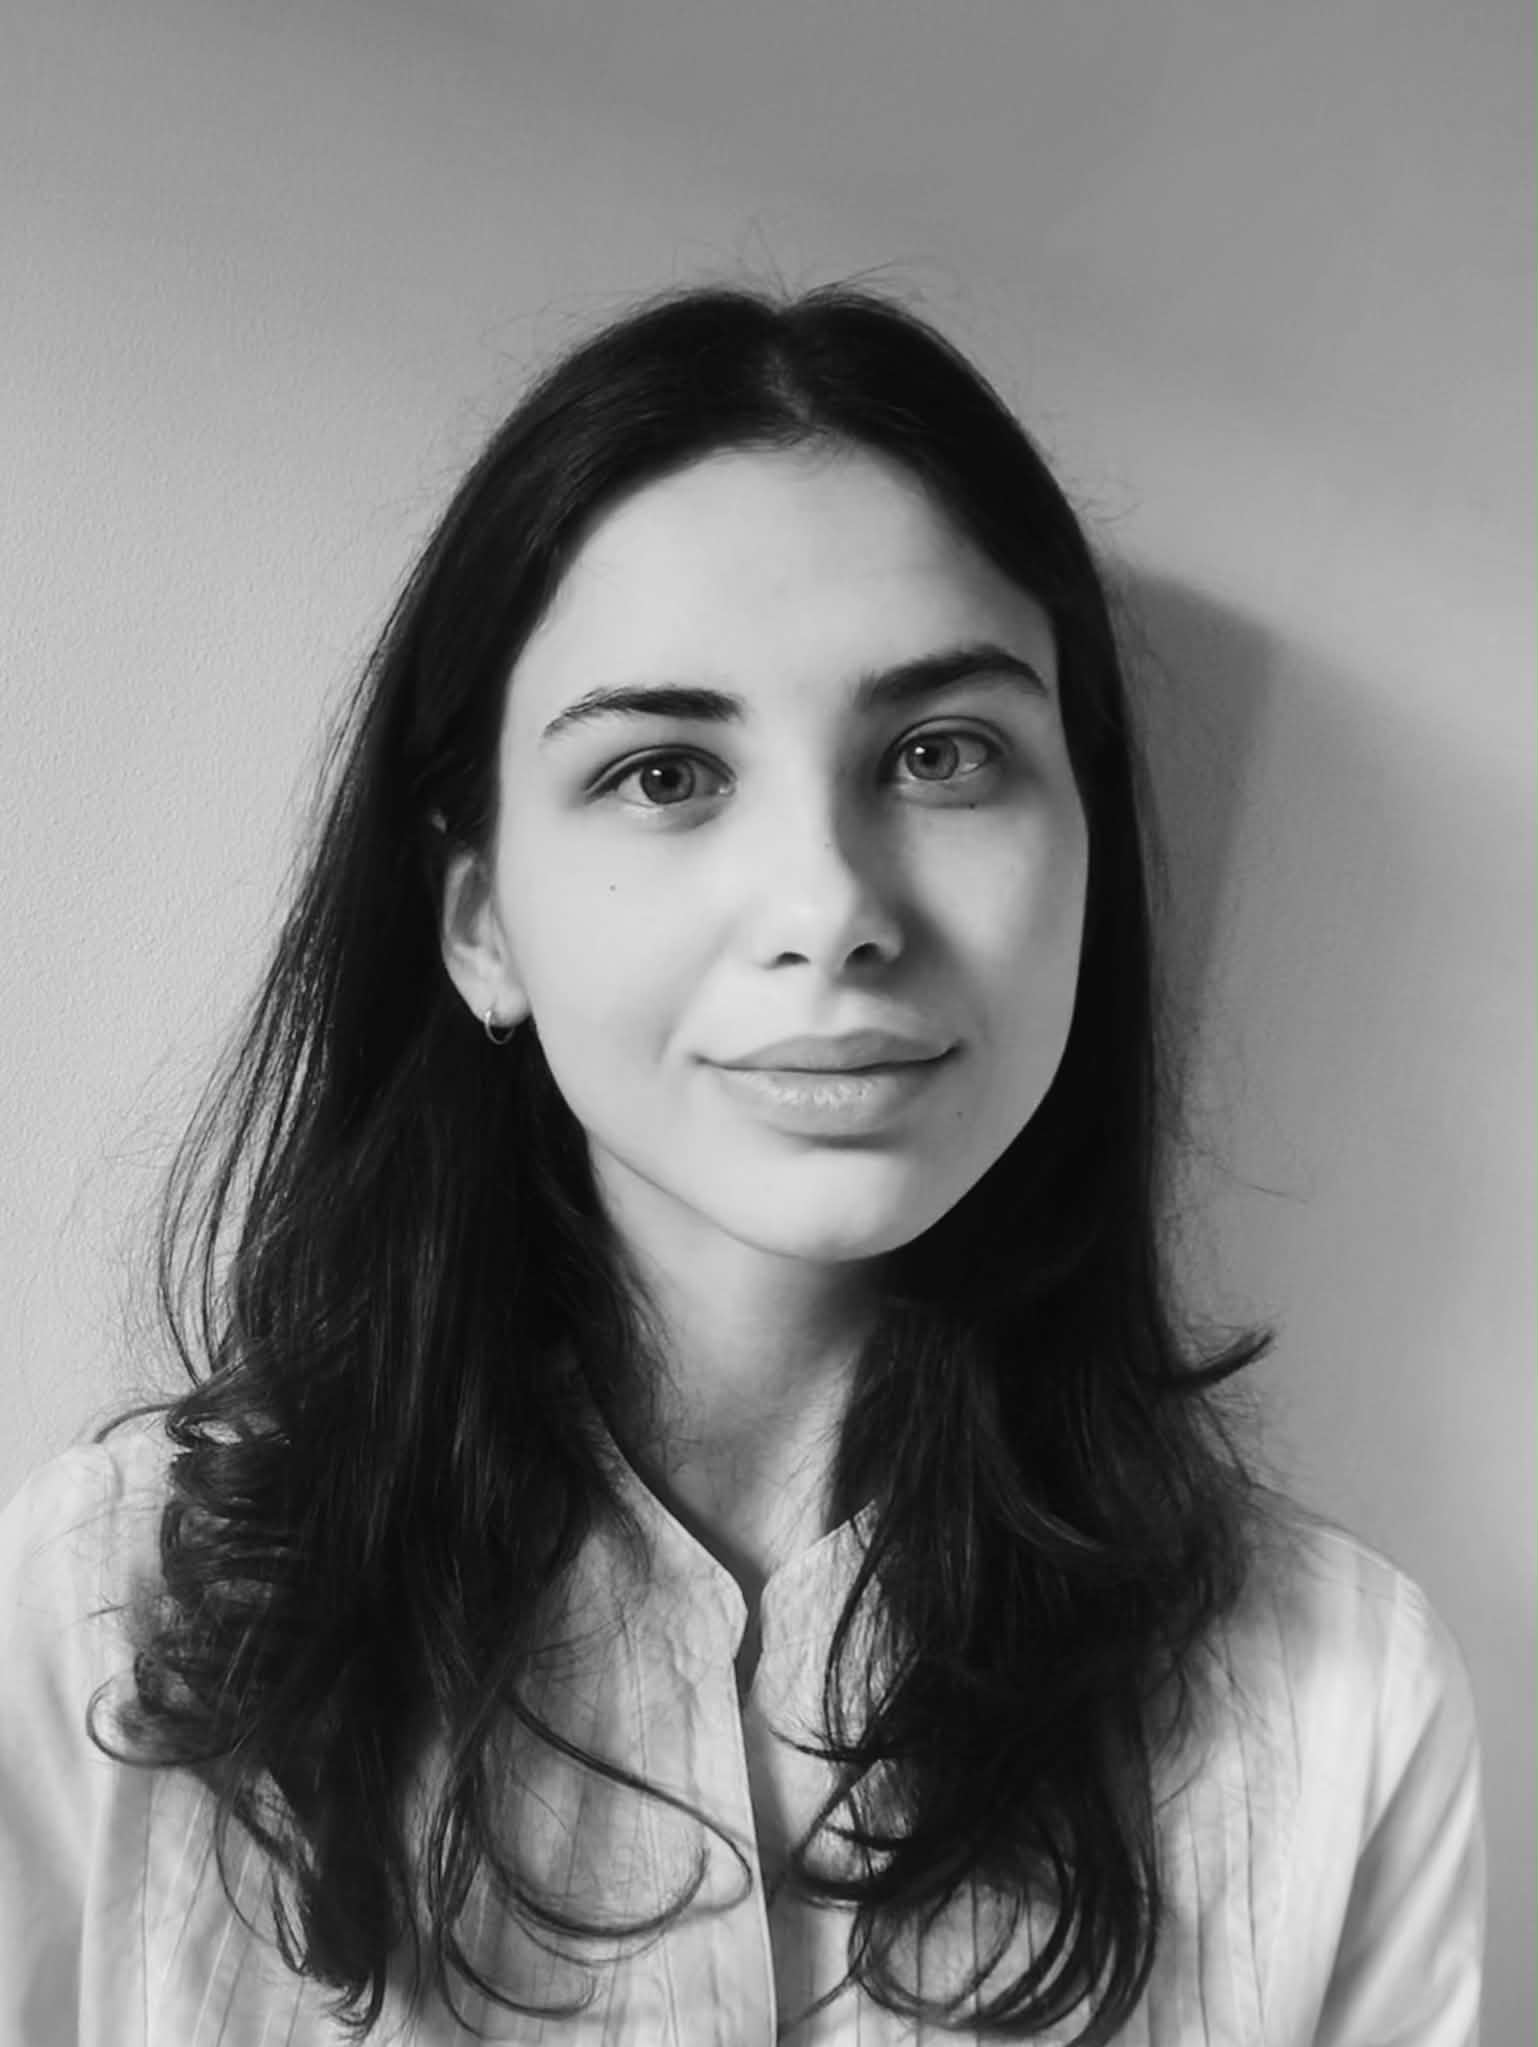
\includegraphics[width=0.7\textwidth]{portretbw.jpg}
    
    
    \vspace{0.3cm}
    \flushleft
    \small

    \textbf{Kontakt} \\
    \vspace{0.1cm}
    Tel.: +48 509 990 122 \\
    E-mail: malgorzata.swiderek33@gmail.com\\
    Warszawa, Polska

    \vspace{0.3cm}
    \textbf{Umiejętności Twarde} \\
    \begin{itemize}[leftmargin=10pt, noitemsep, topsep=1pt]
        \item Java 4/5
        \item JetBrains IDE 4/5
        \item Pakiet Microsoft Office 4/5
        \item Python 3/5
        \item UML 3/5
        \item Autodesk Fusion 3/5
        \item SQL (T-SQL i PL/SQL) 2/5
        \item bash 1/5
        \item C++ 1/5
        \item C\# 1/5

    \end{itemize}

    \vspace{0.3cm}
    \textbf{Języki} \\
    \begin{itemize}[leftmargin=10pt, noitemsep, topsep=1pt]
        \item Polski -- ojczysty
        \item Angielski -- (B1 - B2, w trakcie lektoratu\\na studiach)
        \item Japoński -- podstawowy (A1, w trakcie nauki)

    \end{itemize}

    

    
    \vspace{0.3cm}
    \textbf{Umiejętności Miękkie}
    \begin{itemize}[leftmargin=10pt, noitemsep, topsep=1pt]
        \item Komunikatywność
        \item Szybka nauka
        \item Sumienność
        \item Dbałość o szczegóły
        \item Umiejętność pracy zespołowej

    \end{itemize}
    
    \vspace{0.3cm}
    \textbf{Hobby}
    \begin{itemize}[leftmargin=10pt, noitemsep, topsep=1pt]
        \item Anime
        \item Fotografia
        \item Montaż filmów
        \item Rysunek
        \item Snowboard
        \item Żeglarstwo
    \end{itemize}
    
\end{minipage}

\end{document}
